\chapter{SOM input type study}

\label{chap:som-fv-cifar}

In this chapter, we show an analysis of SOM performance and results with two types of input. Both setups use the same dataset - the CIFAR-10 dataset, but they differ in the type of pre-processing of the data. The first setup uses the CIFAR-10 dataset with no pre-processing. In the second setup, the CIFAR-10 dataset is pre-processed in such a way, that we used the Mean teacher model with properly chosen hyperparameters that provide state-of-the-art performance of the model and calculate feature vectors of each input sample. The mean teacher model was trained with $4000$ labeled samples, other samples were unlabeled. Feature vectors (FV) are representations from the output of the last convolutional layer in the MT model. We compared these two setups to show, that feature vectors of the MT model are suitable for SOM to learn the original dataset representation. And they lead to an even better topology of SOM than the vanilla dataset.

\section{Experiment description}
The task in this experiment was clustering of 10 classes. Dataset CIFAR-10 was already described in section \ref{dataset-cifar10}. It is an image dataset with 10 classes. 
In the first setup, we used this dataset as it is. For the second setup, we trained the Mean teacher model. We used implementation by CuriousAI \cite{curiousai}, which is the original implementation, which was used, when MT was published by Tarvainen in \cite{tarvainen}. In the repository, the read me file says, it is possible to achieve a model with reported results by running script $\texttt{cifar10\_test.py}$. We did that and saved the parameters of the model, which achieved accuracy of $93.68\%$ (student) and $93.88\%$ (teacher). Feature vectors were produced by student model weights. 

For both training types - with CIFAR-10 and with feature vectors - we used the same implementation of SOM and hyperparameters as described in section \ref{pretrained-som}. We investigated several SOM sizes and provided further investigation of SOM metrics (quantization error, winner discrimination and entropy), as well as the map visualization.

\section{Implementation}
Same as in the previous experiment, the SOM model was adapted from repository \cite{som-repo}, which implemented the Self-organizing map using library PyTorch \cite{pytorch}. The implementation of the whole experiment can be found in my repository \cite{dt-mt-repo}, in folder \\ \texttt{pytorch/experiments/cifar-vs-fv-som-visualizations}. The SOM with CIFAR-10 input can be trained by running script \texttt{cifar10-som.py} and the one with feature vector input can be trained by running script \texttt{fv-som.py}. For this second input type, we need to pre-train the MT model, this was done by cloning Mean-teacher repository \cite{curiousai} and running \texttt{python -m experiments.cifar10\_test}, as suggested in \texttt{README.md} file in the Mean-teacher repository, to suggest results of the paper.

\section{Results}
We investigated SOM sizes from $6\times6$ to $15\times15$ neurons in the map.
Each SOM was trained for $100$ epochs. The training curves of SOM metrics are shown in figure \ref{fig:cifar-6n-99ep-stat} and figure \ref{fig:fv-6n-99ep-stat}. In figure \ref{fig:cifar-6n-99ep-stat} we can see the change of metrics during the whole training for $6 \times 6$ map with vanilla CIFAR-10 input. In figure \ref{fig:fv-6n-99ep-stat} we can see the same metrics for $6 \times 6$ map with feature vectors input. 
 Graphs look very similar in their behavior for all SOM sizes in the same input type setup. There is a difference between one setup and another. Quantization error has a different trend. In the FV setup, it looks more nonlinear, in the CIFAR-10 setup trend looks linear. In entropy, CIFAR-10 has increasing direction during the first $80$ epochs and then it drops a little. Entropy in the FV setup has very chaotic progress during the first $60$ epochs, then it increases relatively quickly and reaches similar values as in the CIFAR-10 setup. Winner discrimination is in all cases and during whole training $100\%$, which means, all neurons are chosen as winners for some input. It is reasonable since number of inputs is large.

\begin{figure}[h!]
    \centering
    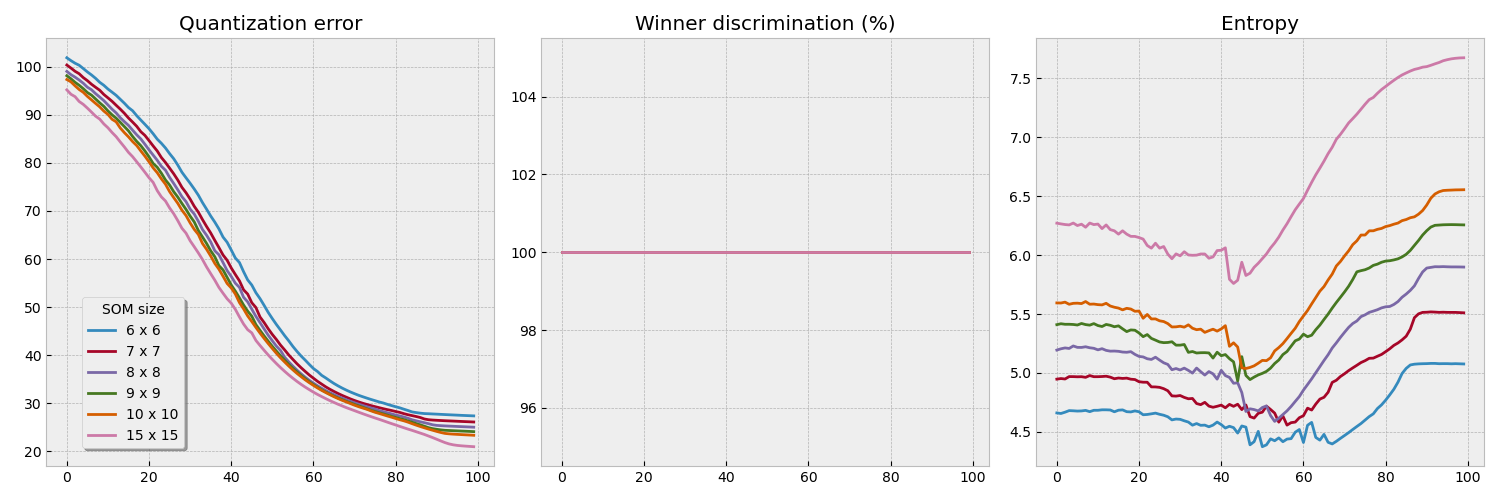
\includegraphics[width=1\textwidth]{figs/fv-som-measures.png}
    \caption{FV input: SOM metrics change during 100 tr. epochs}
    \label{fig:fv-6n-99ep-stat}
\end{figure}

\begin{figure}[h!]
    \centering
    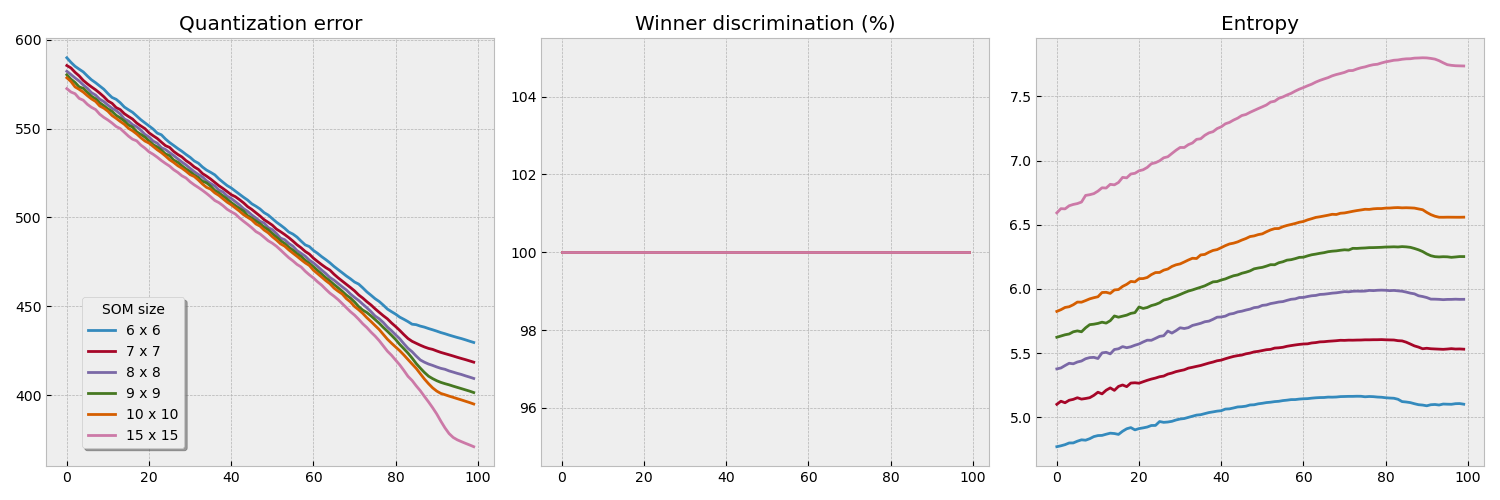
\includegraphics[width=1\textwidth]{figs/cifar-som-measures.png}
    \caption{CIFAR-10 input: SOM metrics change during 100 tr. epochs}
    \label{fig:cifar-6n-99ep-stat}
\end{figure}


For both setups, entropy reached the peak around epoch $85$. Quantization error also begins to decrease slower after circa $85$ epochs. Since by qualitative metrics, this looks like a moment with the best performance of the SOM, we look further into metrics and visualization of the map at this moment of training in the following sections.

\subsection{SOM metrics after 85 epochs}

In this section, we provide SOM metrics after $85$ epochs for investigated SOM sizes. Results are shown in table \ref{tab:som-metrices-85ep}. We can see, that in all cases, winner discrimination is $100\%$, which means, all neurons are chosen as winners during the training process. Entropy in both setups for one chosen size does not differ that much, but we can see, that for CIFAR-10 inputs, SOM entropy is a little higher. When it comes to quantization error, for the feature vector approach, it is much lower, so the prototypes and inputs have a smaller average distance in $n$-dimensional space, than in the opposite approach. 

\begin{table}[h!]
\centering
\begin{tabular}{|c|rrr|rrr|}
\hline
\multicolumn{1}{|l|}{} & \multicolumn{3}{c|}{FV from MT}                                              & \multicolumn{3}{c|}{CIFAR 10}                                            \\ \hline
\multicolumn{1}{|c|}{map size} & \multicolumn{1}{c|}{QE} & \multicolumn{1}{c|}{WD} & \multicolumn{1}{c|}{E} & \multicolumn{1}{c|}{QE} & \multicolumn{1}{c|}{WD} & \multicolumn{1}{c|}{E} \\ \hline
6 $\times$ 6& \multicolumn{1}{r|}{28.17}   & \multicolumn{1}{r|}{100.0\%}   &  5.0 & \multicolumn{1}{r|}{439.87} & \multicolumn{1}{r|}{100.0\%} &  5.12 \\ \hline
7 $\times$ 7& \multicolumn{1}{r|}{27.41}   & \multicolumn{1}{r|}{100.0\%}   &  5.28 & \multicolumn{1}{r|}{430.24} & \multicolumn{1}{r|}{100.0\%} &  5.6 \\ \hline
8 $\times$ 8& \multicolumn{1}{r|}{26.54}   & \multicolumn{1}{r|}{100.0\%}   &  5.64 & \multicolumn{1}{r|}{424.38} & \multicolumn{1}{r|}{100.0\%} &  5.98 \\ \hline
9 $\times$ 9& \multicolumn{1}{r|}{26.04}   & \multicolumn{1}{r|}{100.0\%}   &  5.98 & \multicolumn{1}{r|}{420.8} & \multicolumn{1}{r|}{100.0\%} &  6.33 \\ \hline
10 $\times$ 10& \multicolumn{1}{r|}{25.73}   & \multicolumn{1}{r|}{100.0\%}   &  6.29 & \multicolumn{1}{r|}{417.47} & \multicolumn{1}{r|}{100.0\%} &  6.63 \\ \hline
15 $\times$ 15& \multicolumn{1}{r|}{24.34}   & \multicolumn{1}{r|}{100.0\%}   &  7.53 & \multicolumn{1}{r|}{408.19} & \multicolumn{1}{r|}{100.0\%} &  7.79 \\ \hline

\end{tabular}
\caption{SOM metrics after 85 training epochs}
\label{tab:som-metrices-85ep}
\end{table}

\subsection{Map visualization after 85 epochs}
In this section, we show a visualization of SOM maps after $85$ epochs of training. We choose SOM with size $10\times10$ neurons, to show qualitative difference of results of two input types. Maps are visualized in figure \ref{cifar10-fv-85ep}. In this figure, the color of the neuron represents for which class this neuron was chosen as the winner most frequently, while the size of the neurons represents the percentage of inputs from this major class from all inputs that chose this neuron as their winner - prototype.

\begin{figure*}[h!]
    \centering
    \begin{subfigure}[t]{0.4\textwidth}
        \centering
        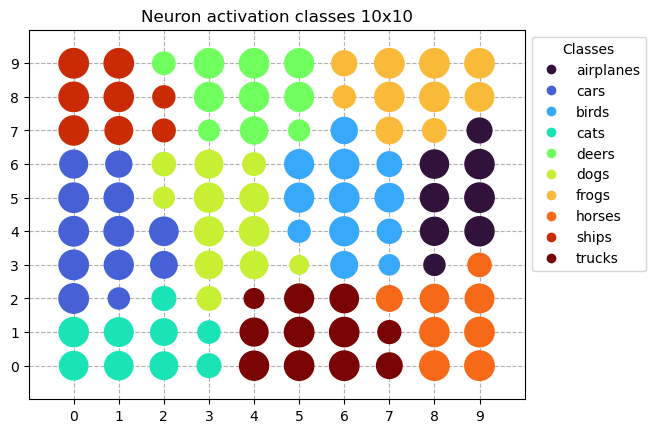
\includegraphics[height=2.2in]{figs/fv-10n-84ep.png}
        \caption{FV input: SOM map visualization}
    \end{subfigure}%
    ~ 
    \begin{subfigure}[t]{0.6\textwidth}
        \centering
        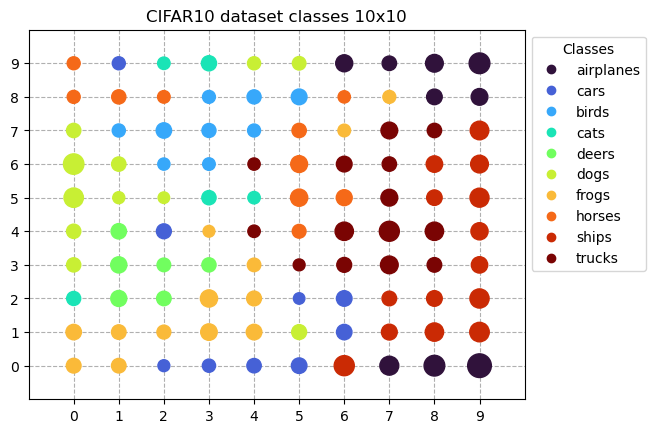
\includegraphics[height=2.2in]{figs/cifar10-10n-84ep-new.png}
        \caption{CIFAR-10 input: SOM map visualization}
    \end{subfigure}

    \caption{Comparison of maps with FV input and CIFAR-10 input}
    \label{cifar10-fv-85ep}
\end{figure*}


On the left side, we can see SOM that was trained from feature vectors of the Mean teacher model. On the right side, there is SOM trained from the unmodified CIFAR-10 dataset. We can see, that clusters on the left map are completely one from another, but on the right side, there are some clear clusters on the right part and in the down left corner of the map, but in the center, there are outliers and disconnected groups of neurons from the same class. Maps differ also in neuron sizes. Since on the left map, prototypes are huge, which means, they properly encode inputs from one class and not many inputs from other classes, in the right map, sizes are very small, so prototype encode more than one class. Based on this visual investigation of map organizations, we can infer that the FV input type improves the clustering ability of SOM.

\begin{figure}[h!]
    \centering
    \includesvg[width=0.95\textwidth]{figs/from-som-weights-10n-99ep.svg}
    \caption{$10 \times 10$ SOM weights visualization}
    \label{fig:som-weights}
\end{figure}


\subsection{SOM neuron weights visualization}
Since SOM neurons are prototypes of inputs and the similarity to input is hidden in neuron weights, which have the same size as input vectors, in vanilla CIFAR-10 input setup, we can visualize weights as images. If a neuron properly represents a class of inputs, we should see some shapes typical for this object in the image. We trained $10 \times 10$ SOM in the same way as before, and visualized its map and weights after $100$ epochs in figures \ref{fig:som-for-weights} and \ref{fig:som-weights}.

\begin{figure}[h!]
    \centering
    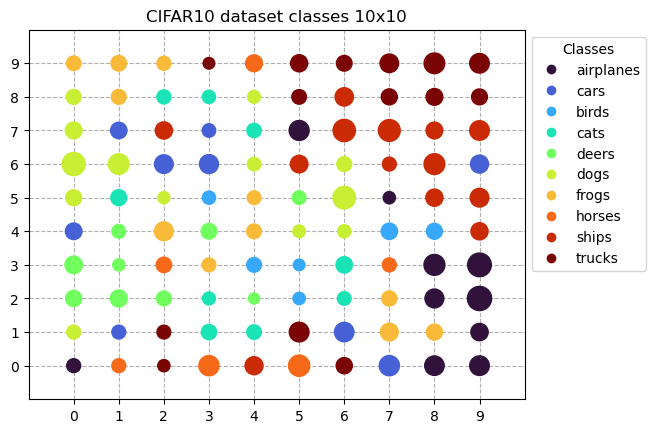
\includegraphics[width=0.6\textwidth]{figs/saved-cifar10-10n-99ep.png}
    \caption{SOM used for weight visualization, map after 100 epochs}
    \label{fig:som-for-weights}
\end{figure}


We can see, that the map is not organized well, there are many outliers, even though we can see some visible clusters of trucks, ships, and airplanes, that cover almost all inputs from the class. When it comes to weight visualization, most of the prototypes do not look like specific objects from one class, however, there are few of them, that look like cars, trucks, horses or frogs. Other classes are not that evidently visible on the visualization.



\section{Discussion}
From this study, we can infer, that using feature vectors as the input of a Self-organizing map is advantageous in few ways. First, the SOM map has better qualitative results, which means smaller quantization error. Second, also qualitative result - visualization - shows a better distribution of data into clusters and fewer outliers. And last, since the feature vector representation has lower dimension than the original inputs, training lasts less time. Based on these observations, we decided to use feature vector inputs in our semi-supervised model with auxiliary SOM loss.

